\section{Introduction}

	\subsection{Goal}
	The main goal of this experiment is to observe the spectral lines of the sodium atom in the visible region to make comments about the physical mechanism of fine structure and verify the theory with experimental data.
	
	\subsection{Theory}
		There are two types of light spectra: Continuous spectrum and discrete spectrum. Continuous spectrum consists of all colors of light and they blend to each other, producing a continuous picture, hence its name. Discrete spectrum consists of only a few colors showing up as lines on the spectrum, not fading into each other, hence its name. The two main physical phenomena we are interested in this experiment, which are diffraction and fine structure.
		
		\subsection{Diffraction Mechanism}
			Diffraction is a useful technique to separate incident light into the wavelength components it is made out of. A transmission diffraction grating was used in this experiment for this exact purpose, separating the wavelengths of incoming light from the sodium discharge tube. The transmission diffraction was achieved by a glass grating with grating spacing that ranges from approximately 1000 nm to 2000 nm.
			\\
			\\
			In general, diffraction mechanism can be written as:
			\begin{equation}
				\delta = n \lambda = d sin \theta
			\end{equation}
			where $\delta$ is the phase difference, $\lambda$ is the wavelength, $d$ is the grating spacing, $\theta$ is the angle and $n$ is the order number.
			\\
			\\
			Viewing the lamp through constant deviation of the grating, the spectral line splitting can be observed. This splitting is called the fine structure and it proves that the energy levels are not the same for different spin orientations for electrons with the same quantum numbers $n$, $l$ and $m$.
		\subsection{Fine Structure}
			The fine structure points to the closely-spaced doublet that can be observed when the spectral lines are viewed under very high resolution. The observation of the fine structure was one of the first evidences of the existence of electron spin. 
			\\
			\\
			This small splitting of the spectral lines is due to the spin orbit interaction between the electron spin and the orbital angular momentum. The magnetic field caused by the orbital angular momentum interacts differently with different spin orientations of the electron. A schematic showing the fine structure in sodium can be seen below.
			\begin{figure}[h!]
				\centering
				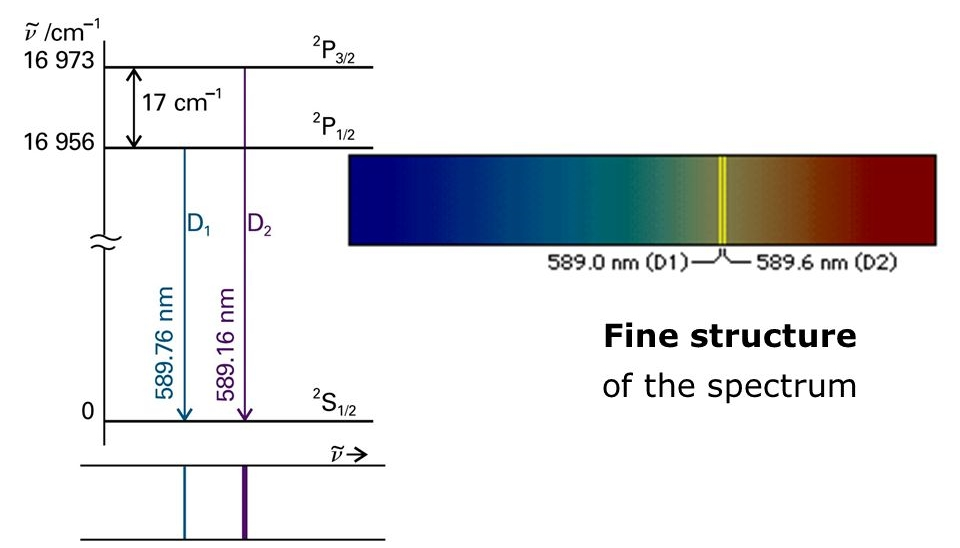
\includegraphics[width=12cm]{images/sodium_fs.jpg}
				\caption{A schematic of fine structure in sodium.}
				\label{fig:na_fs}
			\end{figure}
